\documentclass[a2paper, 12pt]{article}
\usepackage[font={huge, bf}]{caption}
\usepackage{fontspec}
\setmainfont{Arial}
\usepackage{subcaption}
\usepackage{graphicx}
\usepackage{tikz}
\usepackage{tikzsymbols}
\usetikzlibrary{calc,patterns,shapes.geometric}
\usepackage{float}
\usepackage{pdflscape}
\usepackage{geometry}
\geometry{landscape, margin=2cm}
\captionsetup[subfigure]{justification=justified,singlelinecheck=false}
\pagestyle{empty}

\def\centerarc[#1](#2)(#3:#4:#5){\draw[#1] ($(#2)+({#5*cos(#3)},{#5*sin(#3)})$) arc (#3:#4:#5);}

\begin{document}
	\vspace*{\fill}
	\begin{figure}[!htbp]
		\centering
		\begin{subfigure}[b]{0.48\textwidth}
			\caption{Figure 1}
			\centering
			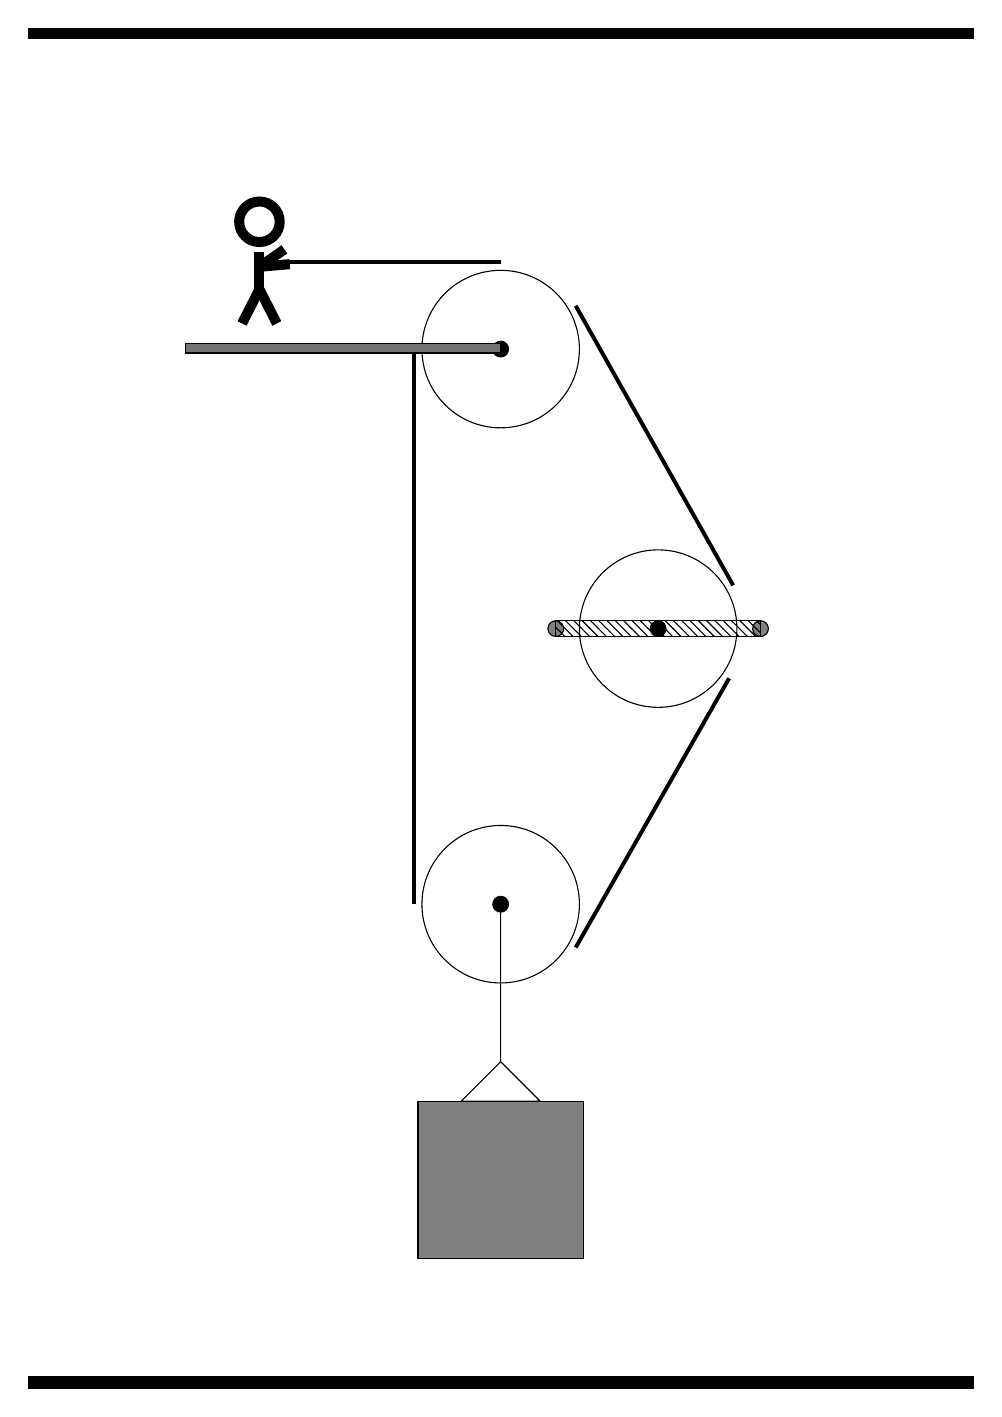
\begin{tikzpicture}
				\draw[fill=black] (-4, 14) rectangle (8, 14.125);
				
				\draw (2, 3.0) circle (1);
				\draw[fill=black] (2, 3.0) circle (0.1);
				
				\draw (2, 10.05) circle (1);
				\draw[fill=black] (2, 10.05) circle (0.1);
				
				\draw[fill=white](4, 6.5) circle (1);
				\draw[fill=black] (4, 6.5) circle (0.1);
				\draw[fill=black!50] (2.7, 6.5) circle (0.1);
				\draw[fill=black!50] (5.3, 6.5) circle (0.1);
				\draw[pattern=north west lines, pattern color=black] (2.7, 6.6) rectangle (5.3, 6.4);
				
				\draw (2, 3.0) -- (2, 1.0) -- (1.5, 0.5) -- (2.5, 0.5) -- (2, 1.0);
				\draw[fill=black!50] (0.95, 0.5) rectangle (3.05, -1.5);
				
				\draw[line width=0.5mm] (0.9, 10) -- (0.9, 3.0);
				\centerarc[line width=0.5mm](2, 3.0)(180:330:1.1);
				\draw[line width=0.5mm](2.9526, 2.45) -- (4.9011, 5.869);
				\centerarc[line width=0.5mm](4, 6.5)(390:325:1.1);
				\draw[line width=0.5mm](4.9526, 7.05) -- (2.9526, 10.6);
				\centerarc[line width=0.5mm](2, 10.05)(30:90:1.1);
				\draw[line width=0.5mm](2, 11.15) -- (-1, 11.15);
				
				\node at (-1, 11.15) {\scriptsize \Strichmaxerl[10][-175][35]};
				\draw[fill=black!55] (-2, 10) rectangle (2, 10.125);
				
				\draw[fill=black] (-4, -3) rectangle (8, -3.15);
			\end{tikzpicture}
		\end{subfigure}
		\hfill
		\begin{subfigure}[b]{0.48\textwidth}
			\caption{Figure 2}
			\centering
			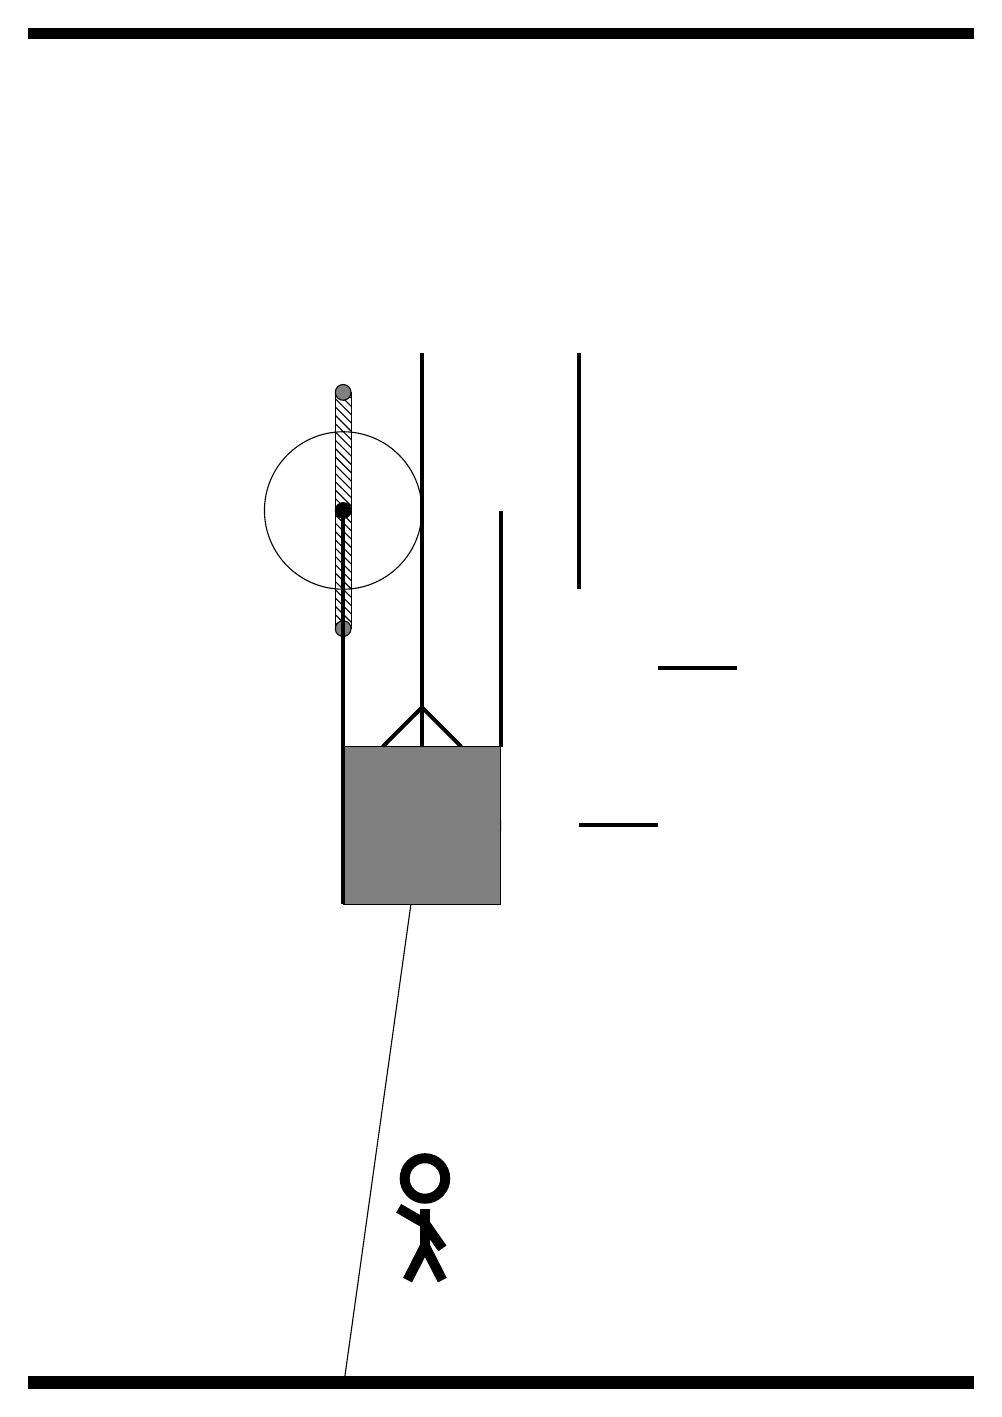
\begin{tikzpicture}
				\draw[fill=black] (-4, 14) rectangle (8, 14.125);
				
				\draw (0,8) circle (1);
				\draw[fill=black] (0,8) circle (0.1);
				\draw[pattern=north west lines, pattern color=black] (-0.1,9.5) rectangle (0.1,6.5);
				\draw[fill=black!50] (0,9.5) circle (0.1);
				\draw[fill=black!50] (0,6.5) circle (0.1);
				
				\draw (1,4) circle (1);
				\draw[fill=black] (1,4) circle (0.1);
				\draw (0,-3.15) -- (1,4);
				
				\draw[line width=0.5mm](0.5,5) --  (1,5.5) -- (1.5,5);
				\draw[fill=black!50] (0, 5) rectangle (2, 3);
				
				\draw[line width = 0.5mm] (1,5) -- (1,10);
				\centerarc[line width = 0.5mm](2,10)(0:180:1);
				\draw[line width = 0.5mm] (3,10) -- (3,7);
				\centerarc[line width = 0.5mm](4,7)(270:180:1);
				\draw[line width = 0.5mm] (4,6) -- (5,6);
				\draw[line width = 0.5mm] (0,3) -- (0,8);
				\centerarc[line width = 0.5mm](1,8)(0:180:1);
				\draw[line width = 0.5mm] (2,8) -- (2,5);
				\centerarc[line width = 0.5mm](3,5)(270:180:1);
				\draw[line width = 0.5mm] (3,4) -- (4,4);
				
				\node at (1, -1) {\scriptsize \Strichmaxerl[10][-30][-55]};
				
				\draw[fill=black] (-4, -3) rectangle (8, -3.15);
			\end{tikzpicture}
		\end{subfigure}
	\end{figure}
		\vspace*{\fill}
\end{document}